\documentclass[12pt,a4paper]{article}
%\documentclass[11pt,UTF8]{article}
%\usepackage{ctex}
\usepackage{tcolorbox}
\usepackage{graphicx}
\usepackage{geometry}
\usepackage{listings}
\usepackage{xcolor}
\usepackage{mathtools}
\usepackage{framed} 
\usepackage{amsfonts}
\usepackage{algpseudocode} 
\usepackage{algorithm}
\usepackage{ulem}
\usepackage{tikz}

\renewcommand{\algorithmicrequire}{ \textbf{Input:}} %Use https://www.overleaf.com/project/6038f72fd2827e6248936428Input in the format of Algorithm
\renewcommand{\algorithmicensure}{ \textbf{Output:}} %Use Output in the format of Algorithm
\definecolor{codegreen}{rgb}{0,0.6,0}
\definecolor{codegray}{rgb}{0.5,0.5,0.5}
\definecolor{codepurple}{rgb}{0.58,0,0.82}
\definecolor{backcolour}{rgb}{0.95,0.95,0.92}

\usepackage{tikz}
\usepackage{tikz-qtree}

\begin{document}
\noindent

%========================================================================
\noindent\framebox[\linewidth]{\shortstack[c]{
\Large{\textbf{Homework 2}}\vspace{1mm}\\
VE216 - Introduction to Signal and Systems, Qiao Heng, Spring 2021}}

\begin{center}

\footnotesize{\color{blue}$*$ Name: Han Yibei\quad\quad\quad\quad\quad Student ID: 519370910123}
\end{center}

\section*{HW Notes:}
\begin{itemize}
    \item Problems where the number of points are followed by an exclamation are basic skill problems and will be graded without partial credit.
    \item \fbox{Box} your final answer. You will be graded on both the final answer and the steps leading to it. Correct intermediate steps will help earn partial credit.
    For full credit, \sout{cross out} any incorrect intermediate step.
    \item If you need to make any additional assumptions, state them clearly.
    \item Legible writing will help when it comes to partial credit.
    \item Simplify your result when possible.
\end{itemize}

\section*{Problems:}
\normalsize
\begin{tcolorbox}[colback = white]
1. One of following two statements is correct, and the other is incorrect. The symbol \fbox{*} denotes \textit{convolution}. $a$ is a constant.
\begin{itemize}
    \item 
    If $y(t)=h(t)*x(t)$ then $y(t-a)=h(t-a)*x(t-a)$;
    \item
    Or if $y(t)=h(t)*x(t)$ then $y(t-a)=h(t)*x(t-a)$.
\end{itemize}
(a) [4!] Give a simple proof of the correct statement.\\
(b) [3!] Give a simple counterexample for the incorrect statement.\\
(c) [3!] Repeat (a) and (b) for the following two statements. The symbol \fbox{$\cdot$} denotes \textit{multiplication}.
 
\begin{itemize}
    \item if $y(t)=h(t)\cdot x(t) $ then $y(t-a)=h(t-a)\cdot x(t-a)$;
    \item
    Or if $y(t)=h(t)\cdot x(t)$ then $y(t-a)=h(t)\cdot x(t-a)$.
\end{itemize}
Be careful with the notation $h(t)*x(t)$. More precise notation is $(h*x)(t)$, which makes it clear that convolution is an operation on two signals, not a point-wise operation like multiplication. For question (a), can you utilize the property of delay property of convolution?

\end{tcolorbox}

\begin{tcolorbox}
\normalsize
\textcolor{blue}{Answer:\\
(a) The \fbox{second} one is right 
$$\begin{aligned}
    y(t)&=h(t)*x(t)=\int_{-\infty}^\infty h(\tau)x(t-\tau)d\tau\\\rightarrow y(t-a&)=\int_{-\infty}^\infty h(\tau)x(t-\tau+a)d(\tau)=h(t)*x(t-a)
\end{aligned}$$
(b) let x(t)=$\delta(t)$ and h(t)=u(t) then
$$y(t)=h(t)*x(t)=u(t)\rightarrow y(t-a)=u(t-a)$$
$$h(t-a)*x(t-a)=u(t-a)*\delta(t-a)=u(t-2a)\neq y(t-a)$$
(c) The \fbox{first} one is right
$$
\begin{aligned}
    y(t-a)&=y(t)*\delta(t-a)=(h(t)x(t))*\delta(t-a)\\
    &=h(t)*\delta(t-a)\cdot x(t)*\delta(t-a)=h(t-a)x(t-a)
\end{aligned}
$$
let x(t)=$\delta(t)$ and h(t)=u(t) and a<0 then
$$y(t)=h(t)x(t)=\delta(t)\rightarrow y(t-a)=\delta(t-a)$$
$$h(t)x(t-a)=0 \neq y(t-a)$$
}
\end{tcolorbox}

\begin{tcolorbox}[colback = white]
2. Let $y(t)=(x*h)(t)$. Show the following properties of convolution.\\
(a) [5!] $\int_{-\infty}^{\infty} y(t) d t=\left[\int_{-\infty}^{\infty} x(t) d t\right]\left[\int_{-\infty}^{\infty} h(t) d t\right]$;\\
(b) [5!] $\frac{d^n}{d t^n} y(t)=\left[\frac{d^n}{d t^n} x(t)\right] * h(t)=x(t) *\left[\frac{d^n}{d t^n} h(t)\right]$;
\end{tcolorbox}

\begin{tcolorbox}
\normalsize
\textcolor{blue}{Answer:\\
(a)$$
\begin{aligned}
    \int_{-\infty}^\infty y(t)d&t=\int_{-\infty}^\infty \int_{-\infty}^\infty x(\tau) h(\tau-a) d\tau\\
    &=\int_{-\infty}^\infty \int_{-\infty}^\infty x\tau h(t-\tau) dt d\tau\\
    &=\int_{-\infty}^\infty  x(\tau) \int_{-\infty}^\infty h(t-\tau) d(t-\tau) d\tau\\
    &=[\int_{-\infty}^\infty x(\tau) d\tau][\int_{-\infty}^\infty h(m) dm]\\
    &=\fbox{$\int_{-\infty}^\infty x(t) dt][\int_{-\infty}^\infty h(t) dt]$}
\end{aligned}
$$
(b)$$
\begin{aligned}
    \frac{d^n}{dt^n}y(t)&=\frac{d^n}{dt^n} \int_{-\infty}^\infty x(\tau) h(t-\tau) d\tau\\
    &=\int_{-\infty}^\infty \frac{d^n}{dt^n} x(\tau) h(t-\tau) d\tau\\
    &=\int_{-\infty}^\infty [\frac{d^n}{dt^n} x(\tau)] h(t-\tau) d\tau\\
    &=\fbox{$[\frac{d^n}{dt^n} x(t)]*h[t]$}
\end{aligned}
$$
similarly, we can get \fbox{$\frac{d^n}{dt^n}y(t)=x(t)\frac{d^n}{dt^n} h(t)]$}
}
\end{tcolorbox}

\begin{tcolorbox}[colback = white]
3. Often we will be convolving two signals that are zero everywhere except over some finite range (called \textbf{finite support} signals). Suppose $x_{1}(t)$ is non-zero over the range $a\leq t\leq b$ and that $x_{2}(t)$ is non-zero over the range $c\leq t\leq d$. Suppose $y(t) = x_{1}(t) * x_{2}(t)$.\\
(a) [5!] Find the range of values of t for which y(t) is possibly non-zero.\\
(b) [10!] Compute $rect((t-2)/4)*rect((t+1)/6)$ (express answer with braces and carefully sketch). Check your result with part (a).
\end{tcolorbox}

\begin{tcolorbox}
\normalsize
\textcolor{blue}{Answer:\\
(a) $y(t)=\int_{-\infty}^\infty x_1(\tau)x_2(t-\tau)dt$
we need to get\\
$a\leq\tau\leq b$ and $c\leq t-\tau \leq d$, we can get $a+c\leq t\leq b+d$
(b) $$y(t)=\int_{-\infty}^\infty rect(\frac{\tau-2}{4}) rect(\frac{t-\tau+1}{6})$$ 
for $x_1$, $0\leq\tau\leq 4$, for $x_2$, $t-2\leq\tau\leq t+4$
$$\fbox{g(t)}=
\begin{cases}
    4+t & -4<t \leq 0 \\
    4 & 0<t \leq 2 \\
    6-t & 2<t \leq 6 \\
    0 & t\leq -4 \text{ and } 6\leq t
\end{cases}$$
\begin{figure}[H]
    \centering
    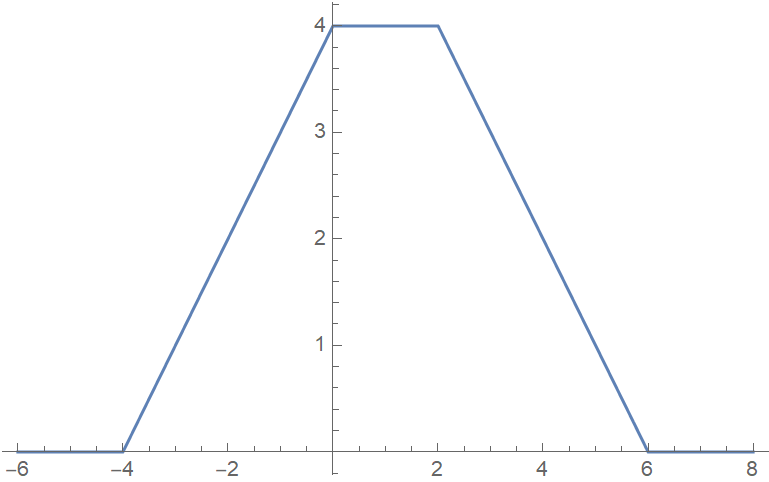
\includegraphics[width=10cm]{3b.jpg}
\end{figure}
}
\end{tcolorbox}

\newpage
\begin{tcolorbox}[colback = white]
4. [15!] Consider a LTI system. Let its impulse response h(t) be the triangular pulse shown below, and x(t) be the \textit{impulse train}\\
$$
x(t)=\sum_{n=-\infty}^{\infty} \delta(t-n T)
$$
SKETCH $y(t)=x(t)*h(t)$ for T=2, 1.5 and 1. (No formulae are needed though you still want to label your graphs clearly.)\\
%\begin{center}
%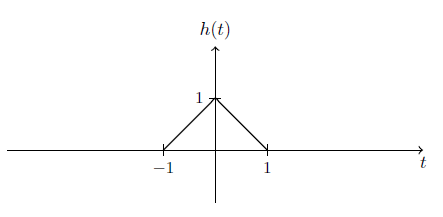
\includegraphics[scale=0.5]{problem4.png}
%\end{center}
\begin{center}
    \begin{tikzpicture}
    \draw[->] (-3,0) -- (3,0) node[right]{$t$};
    \draw[->] (0,-0.1) -- (0,2) node[above]{$h(t)$};
    \draw[-] (-1,0) -- (1,1); 
    \draw[-] (1,1) -- (1,0);
    \draw (-1,0)node[below]{-1}--(-1,0.1);
    \draw (1,0)node[below]{1}--(1,0.1);
    \draw (0,1)--(0.1,1) node[left]{1};
    \draw (0,0) node[below]{0};
    \end{tikzpicture}
\end{center}
\end{tcolorbox}

\begin{tcolorbox}
\normalsize
\textcolor{blue}{Answer:\\
$$y(t)=h(t)*x(t)=\sum_{n=-\infty}^\infty h(t-nT)$$
\begin{figure}[H]
    \centering
    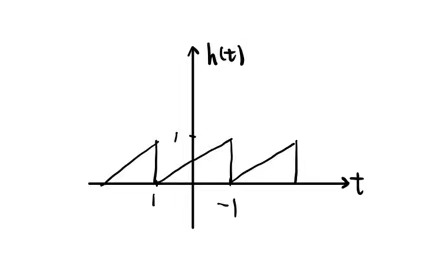
\includegraphics[width=8cm]{41.jpg}
\end{figure}
\begin{figure}[H]
    \centering
    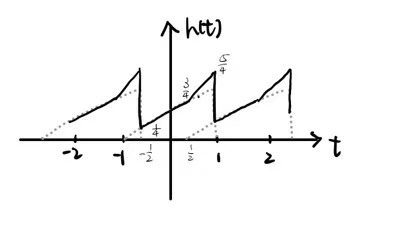
\includegraphics[width=8cm]{42.jpg}
\end{figure}
\begin{figure}[H]
    \centering
    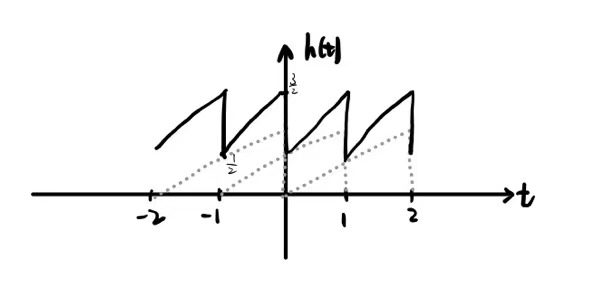
\includegraphics[width=8cm]{43.jpg}
\end{figure}
}
\end{tcolorbox}


\begin{tcolorbox}[colback = white]
5. [2$\times$5!] Consider an LTI system whose response to the signal $x_{1}(t)$ is the signal $y_{1}(t)$ which are illustrated
below.\\
(a) Determine and sketch carefully the response of the system to the input $x_{2}(t)$ depicted below.\\
(b) Determine and sketch carefully the response of the system to the input $x_{3}(t)$ depicted below.\\
%\begin{center}
%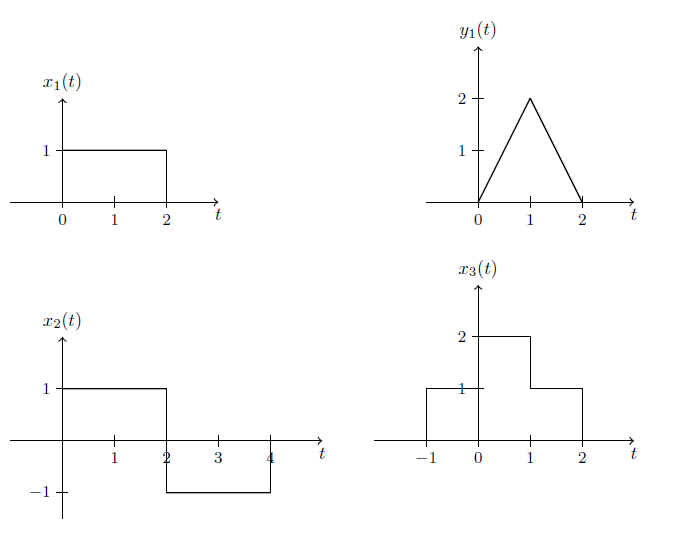
\includegraphics[scale=1.0]{problem5.png}
%\end{center}
\begin{center}
    \begin{tikzpicture}
    \draw[->] (-6,0) -- (-2,0) node[right]{$t$};
    \draw[->] (-5,-0.1) -- (-5,2) node[right]{$x_1(t)$};
    \draw[-] (-5,1) -- (-3,1);
    \draw[-] (-3,1) -- (-3,0);
    \draw (-5,0)node[below]{0}--(-5,0.1);
    \draw (-4,0)node[below]{1}--(-4,0.1);
    \draw (-3,0)node[below]{2}--(-3,0.1);
    \draw (-5,1)node[left]{1}--(-4.9,1);
    \draw[->] (2,0) -- (6,0) node[right]{$t$};
    \draw[->] (3,-0.1) -- (3,2) node[right]{$y_1(t)$};
    \draw[-] (3,0) -- (4,1);
    \draw[-] (4,1) -- (5,0);
    \draw (3,0)node[below]{0}--(3,0.1);
    \draw (4,0)node[below]{1}--(4,0.1);
    \draw (5,0)node[below]{2}--(5,0.1);
    \draw (3,1)node[left]{1}--(3.1,1);
    \end{tikzpicture}
\end{center}
\begin{center}
    \begin{tikzpicture}
    \draw[->] (-6,0) -- (-1,0) node[right]{$t$};
    \draw[->] (-5,-2) -- (-5,2) node[right]{$x_2(t)$};
    \draw[-] (-5,1) -- (-4,1);
    \draw[-] (-4,1) -- (-4,0);
    \draw[-] (-3,0) -- (-3,-1);
    \draw[-] (-3,-1) -- (-2,-1);
    \draw[-] (-2,-1) -- (-2,0);
    \draw (-4,0)node[below]{1}--(-4,0.1);
    \draw (-3,0)node[below]{2}--(-3,0.1);
    \draw (-2,0)node[below]{3}--(-2,0.1);
    \draw (-5,1)node[left]{1}--(-4.9,1);
    \draw (-5,-1)node[left]{-1}--(-4.9,-1);
    \draw[->] (1,0) -- (6,0) node[right]{$t$};
    \draw[->] (3,-0.1) -- (3,3) node[right]{$x_3(t)$};
    \draw (2,0)node[below]{-1}--(2,0.1);
    \draw (3,0)node[below]{0}--(3,0.1);
    \draw (4,0)node[below]{1}--(4,0.1);
    \draw (5,0)node[below]{2}--(5,0.1);
    \draw (3,1)node[left]{1}--(3.1,1);
    \draw (3,2)node[left]{2}--(3.1,2);
    \draw[-] (2,0) -- (2,1);
    \draw[-] (2,1) -- (3,1);
    \draw[-] (3,2) -- (4,2);
    \draw[-] (4,2) -- (4,1);
    \draw[-] (4,1) -- (5,1);
    \draw[-] (5,1) -- (5,0);
    \end{tikzpicture}
\end{center}
\end{tcolorbox}

\begin{tcolorbox}
\normalsize
\textcolor{blue}{Answer:\\
(a) $x_2(t)=x_1(t)-x_1(t-1)\rightarrow y_2(t)=y_1(t)-y_1(t-1)$\\
(b) $x_2(t)=x_1(t)+x_1(t+1)\rightarrow y_2(t)=y_1(t)+y_1(t+1)$
\begin{figure}[H]
    \centering
    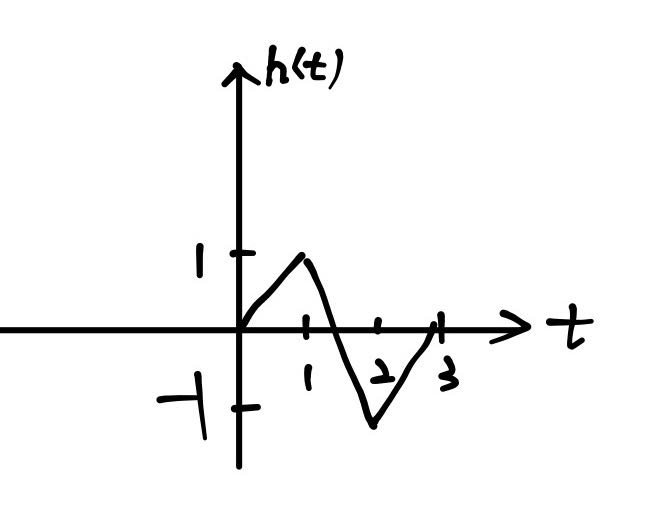
\includegraphics[width=8cm]{51.jpg}
\end{figure}
\begin{figure}[H]
    \centering
    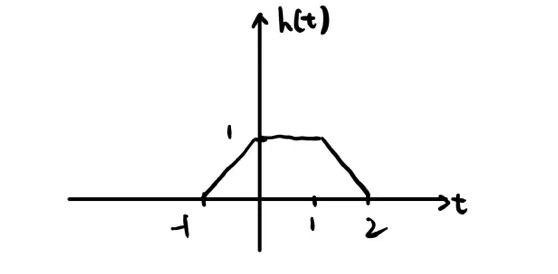
\includegraphics[width=8cm]{52.jpg}
\end{figure}}
\end{tcolorbox}

\begin{tcolorbox}[colback = white]
6. [10!] The triangular pulse is defined as $tri(t)=(1-|t|)rect(t/2)$. Compute $x(t)=tri(t/2)*rect(\frac{t-1}{2})$. Express your answer using braces, and carefully sketch.

\end{tcolorbox}

\begin{tcolorbox}
\normalsize
\textcolor{blue}{Answer:\\
$x(t)=(1-|\frac{t}{2}|)rect(\frac{t}{4})*rect(\frac{t-1}{2})=\int_{-\infty}^\infty (1-|\frac{\tau}{2}|)rect(\frac{\tau}{4})rect(\frac{t-\tau-1}{2})d\tau$\\
(1)-2<t<0 $x(t)=\int_{-2}^t(1+\frac{\tau}{2})d\tau=\frac{t^2}{4}+t+1$\\
(2)0$\leq$ t<2 $x(t)=\int_0^t(1-\frac{\tau}{2})d\tau+\int_{t-2}^0(1+\frac{\tau}{2})d\tau=-\frac{t^2}{2}+t+1$\\
(3)2$\leq$ t $\leq$4 $x(t)=\int_{t-2}^2(1-\frac{\tau}{2})d\tau=\frac{t^2}{4}-2t+4$\\
(4) others 0
$$\fbox{g(t)}=
\begin{cases}
    \frac{t^2}{4}+t+1 & -2<t<0 \\
    -\frac{t^2}{2}+t+1 & 0\leq t<2 \\
    \frac{t^2}{4}-2t+4 & 2\leq t \leq4 \\
    0 & t\leq others
\end{cases}$$
\begin{figure}[H]
    \centering
    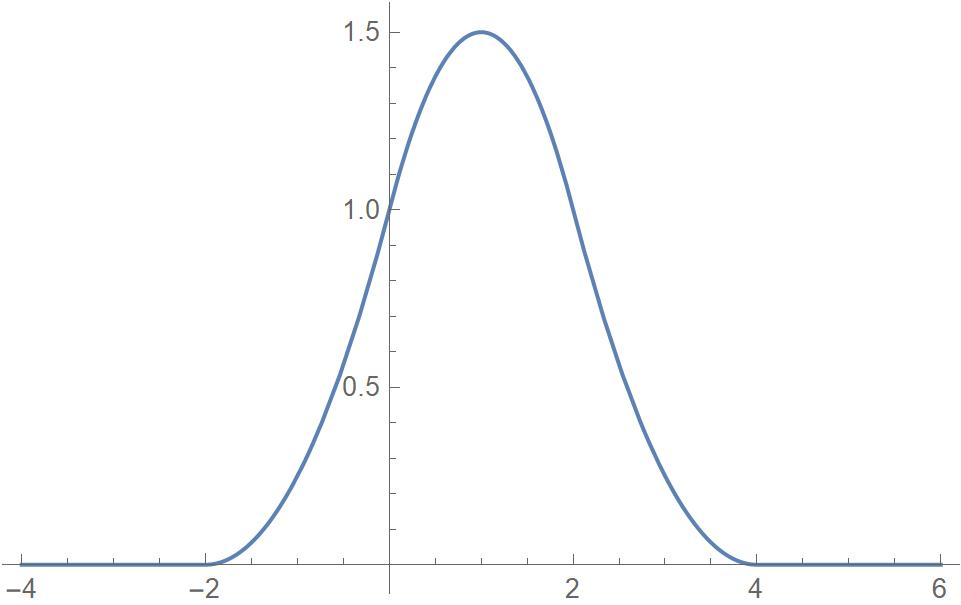
\includegraphics[width=10cm]{6b.jpg}
\end{figure}
}
\end{tcolorbox}
\newpage
\begin{tcolorbox}[colback = white]

7. [4$\times$4!] Find the impulse response of the following LTI systems and further determine whether they are causal, stable and static.\\
(a) $y(t)=\int_{-\infty}^{t}(\tau-t) e^{-2(t-\tau)} x(\tau) d \tau$\\
(b) $y(t)=\int_{t-2}^{t} e^{-(t-\tau)} x(\tau) d \tau$\\
(c) $y(t)=\int_{-\infty}^{t}\left[\int_{-\infty}^{s} x(\tau-5) d \tau\right] d s$\\
(d) $y(t)=\int_{-3}^{3} \tau^{2} x(t-\tau) d \tau+\int_{-\infty}^{t+1}(t-\tau+3)^{-2} x(\tau) d \tau$
\end{tcolorbox}
\begin{tcolorbox}
\normalsize
\textcolor{blue}{Answer:\\
(a) $y(t)=\int_{-\infty}^t(\tau-t)e^{-2(t-\tau)}x(\tau)d\tau=\int_{-\infty}^\infty(\tau-t)e^{-2(t-\tau)}u(t-\tau)x(\tau)d\tau\\~~~~~~~~~~~=x(t)*(-te^{-2t}u(t))\rightarrow h(t)=-te^{-2t}u(t)$\\
\textbf{Casual:} It is casual because h(t)=0 when t<0\\
\textbf{Stable:} It is stable because $\int_{-\infty}^\infty |-te^{-2t}u(t)|dt=\int_0^\infty te^{-2t}dt=\frac{1}{4}\neq\infty$\\
\textbf{Static:} It is not static because h(t)$\neq$k$\delta$(t)\\
So it is casual, stable and not static.\\
\\
(b) $y(t)=\int_{t-2}^{t} e^{-(t-\tau)} x(\tau) d \tau=\int_{-\infty}^{\infty} e^{-(t-\tau)} x(\tau)u(\tau-t+2)u(t-\tau) d \tau$\\
$h(t)= e^{-t}u(2-t)u(t)$\\
\textbf{Casual:} It is casual because h(t)=0 when t<0\\
\textbf{Stable:} It is stable because $\int_{-\infty}^\infty |e^{-t}u(2-t)u(t)|dt=\int_0^2 e^{-t}dt=1-e^{-2}\neq\infty$\\
\textbf{Static:} It is not static because h(t)$\neq$k$\delta$(t)\\
So it is \fbox{casual, stable and not static}.\\
\\
(c) $y(t)=\int_{-\infty}^{t}[\int_{-\infty}^{s} x(\tau-5) d \tau] ds=\int_{-\infty}^{t}[\int_{-\infty}^{\infty} x(\tau-5)u(s-\tau) d \tau] ds\\~~~~~~~~~~~=\int_{-\infty}^{t}x(s)u(s-5) ds=\int_{-\infty}^{\infty}x(s)u(s-5)u(t-s)ds \\
~~~~~~~~~~~\rightarrow h(t)=u(t-5)*u(t)=(t-5)u(t-5)$\\
\textbf{Casual:} It is casual because h(t)=0 when t<0\\
\textbf{Stable:} It is not stable because $\int_{-\infty}^\infty |h(t)|dt=\infty$\\
\textbf{Static:} It is not static because h(t)$\neq$k$\delta$(t)\\
So it is \fbox{casual, not stable and not static
}.\\
(d) \\$
\begin{aligned}
    y(t)&=\int_{-3}^{3} \tau^{2} x(t-\tau) d \tau+\int_{-\infty}^{t+1}(t-\tau+3)^{-2} x(\tau) d \tau\\
    &=x(t)*(u(t+3)u(3-t)t^2)+x(t)*(u(t+1)(t+3)^{-2})\\
    \rightarrow&h(t)=u(t+3)u(3-t)t^2+u(t+1)(t+3)^{-2}
\end{aligned}
$\\
\textbf{Casual:} It is not casual because h(t)$\neq$0 when t<0\\
\textbf{Stable:} It is stable because $\int_{-\infty}^\infty |h(t)|dt<\infty$\\
\textbf{Static:} It is not static because h(t)$\neq$k$\delta$(t)\\
So it is \fbox{not casual, stable and not static}.
}
\end{tcolorbox}

\begin{tcolorbox}[colback = white]
8. [10!] Consider an LTI system S and a signal $x(t)=e^{-5t}u(t-1)$. If
$x(t) \rightarrow y(t)$
and
$$\frac{d}{dt}x(t) \rightarrow -5y(t)+e^{-t}u(t) $$
determine the impulse response h(t) of S.
\end{tcolorbox}
\begin{tcolorbox}
\normalsize
\textcolor{blue}{Answer:\\
$\frac{d}{dt}x(t)=-5e^{-5t}u(t-1)+e^{-5t}\delta(t-1)$\\
Since it's an LTI system, we cna know that $e^{-5t}\delta(t-1)\rightarrow e^{-t}u(t)$\\
Since $\delta(t-1)$ is only suitable for t=1: $e^{-5}\delta(t-1)\rightarrow e^{-t}u(t)$\\
then $\delta(t-1)\rightarrow e^{-t+5}u(t)$\\
$h(t-1)=e^{-t+5}u(t)\rightarrow h(t)=\fbox{$e^{-t+4}u(t+1)$}$
}

\end{tcolorbox}

\begin{tcolorbox}[colback = white]
9. [4!] Find the expression of response of the CT system described by the linear constant-coefficient differential equation.
$$\frac{d}{dt}y(t)+10y(t)=2x(t)$$
where
$$y(0)=1; x(t)=u(t)$$
\end{tcolorbox}
\begin{tcolorbox}
\normalsize
\textcolor{blue}{Answer:\\
First, we found the solution for $\frac{d}{dt}y(t)+10y(t)=0$ and $y_h(t)=C e^{-10t}$\\
x(t)=u(t), so $\frac{d}{dt}x(t)=0$ for x>0, so $y_p=P$\\
$-10C e^{-10t}+10C e^{-10t}+10P=2$, so $P=\frac{1}{5}$\\
$y(0)=1\rightarrow C+\frac{1}{5}=1\rightarrow C=\frac{4}{5}$\\
$y=y_h+y_p=\frac{4}{5} e^{-10t}+\frac{1}{5}$, but y is 0 when $y\leq 0$, so $y(t)=(\frac{4}{5} e^{-10t}+\frac{1}{5})u(t)$\\
$h(t)=\frac{d}{dt}y(t)=\fbox{$-8e^{-10t}u(t)+\delta(t)$}$
}

\end{tcolorbox}
%========================================================================
\end{document}

